% Options for packages loaded elsewhere
\PassOptionsToPackage{unicode}{hyperref}
\PassOptionsToPackage{hyphens}{url}
%
\documentclass[
]{article}
\usepackage{amsmath,amssymb}
\usepackage{lmodern}
\usepackage{iftex}
\ifPDFTeX
  \usepackage[T1]{fontenc}
  \usepackage[utf8]{inputenc}
  \usepackage{textcomp} % provide euro and other symbols
\else % if luatex or xetex
  \usepackage{unicode-math}
  \defaultfontfeatures{Scale=MatchLowercase}
  \defaultfontfeatures[\rmfamily]{Ligatures=TeX,Scale=1}
\fi
% Use upquote if available, for straight quotes in verbatim environments
\IfFileExists{upquote.sty}{\usepackage{upquote}}{}
\IfFileExists{microtype.sty}{% use microtype if available
  \usepackage[]{microtype}
  \UseMicrotypeSet[protrusion]{basicmath} % disable protrusion for tt fonts
}{}
\makeatletter
\@ifundefined{KOMAClassName}{% if non-KOMA class
  \IfFileExists{parskip.sty}{%
    \usepackage{parskip}
  }{% else
    \setlength{\parindent}{0pt}
    \setlength{\parskip}{6pt plus 2pt minus 1pt}}
}{% if KOMA class
  \KOMAoptions{parskip=half}}
\makeatother
\usepackage{xcolor}
\IfFileExists{xurl.sty}{\usepackage{xurl}}{} % add URL line breaks if available
\IfFileExists{bookmark.sty}{\usepackage{bookmark}}{\usepackage{hyperref}}
\hypersetup{
  pdftitle={Budget Overruns: First Implementation of QuickPay (2009-2012)},
  hidelinks,
  pdfcreator={LaTeX via pandoc}}
\urlstyle{same} % disable monospaced font for URLs
\usepackage[margin=1in]{geometry}
\usepackage{graphicx}
\makeatletter
\def\maxwidth{\ifdim\Gin@nat@width>\linewidth\linewidth\else\Gin@nat@width\fi}
\def\maxheight{\ifdim\Gin@nat@height>\textheight\textheight\else\Gin@nat@height\fi}
\makeatother
% Scale images if necessary, so that they will not overflow the page
% margins by default, and it is still possible to overwrite the defaults
% using explicit options in \includegraphics[width, height, ...]{}
\setkeys{Gin}{width=\maxwidth,height=\maxheight,keepaspectratio}
% Set default figure placement to htbp
\makeatletter
\def\fps@figure{htbp}
\makeatother
\setlength{\emergencystretch}{3em} % prevent overfull lines
\providecommand{\tightlist}{%
  \setlength{\itemsep}{0pt}\setlength{\parskip}{0pt}}
\setcounter{secnumdepth}{5}
\usepackage{booktabs,longtable,dcolumn} \usepackage{multirow,array} \usepackage{wrapfig,float} \floatplacement{figure}{H}
\ifLuaTeX
  \usepackage{selnolig}  % disable illegal ligatures
\fi

\title{Budget Overruns: First Implementation of QuickPay (2009-2012)}
\author{}
\date{\vspace{-2.5em}Sep 26, 2021}

\begin{document}
\maketitle

\hypertarget{note}{%
\section{Note}\label{note}}

\begin{itemize}
\tightlist
\item
  Sample restricted to projects for which start dates matches the one in
  API

  \begin{itemize}
  \tightlist
  \item
    This is done by using first reported ``action\_date'' and
    ``date\_signed''
  \end{itemize}
\item
  Below is the definition of \texttt{base\_and\_all\_options\_value}
  from the data dictionary:

  \begin{itemize}
  \tightlist
  \item
    The change (from this transaction only) to the potential contract
    value (i.e., the base contract and any exercised or unexercised
    options).
  \end{itemize}
\item
  This means that every observation in raw data shows incremental change
  from previous budget. So some of the values can be zero.
\item
  We, therefore, need to calculate the new budget at each point in time
  (by adding all previous values). We did this in the resampling step,
  but mentioning here for reference.
\item
  This is different from calculation of delays, where
  \texttt{period\_of\_performance\_current\_end\_date} indicated the new
  deadline of the project.
\end{itemize}

\hypertarget{budget-overrun-over-time}{%
\section{Budget Overrun over Time}\label{budget-overrun-over-time}}

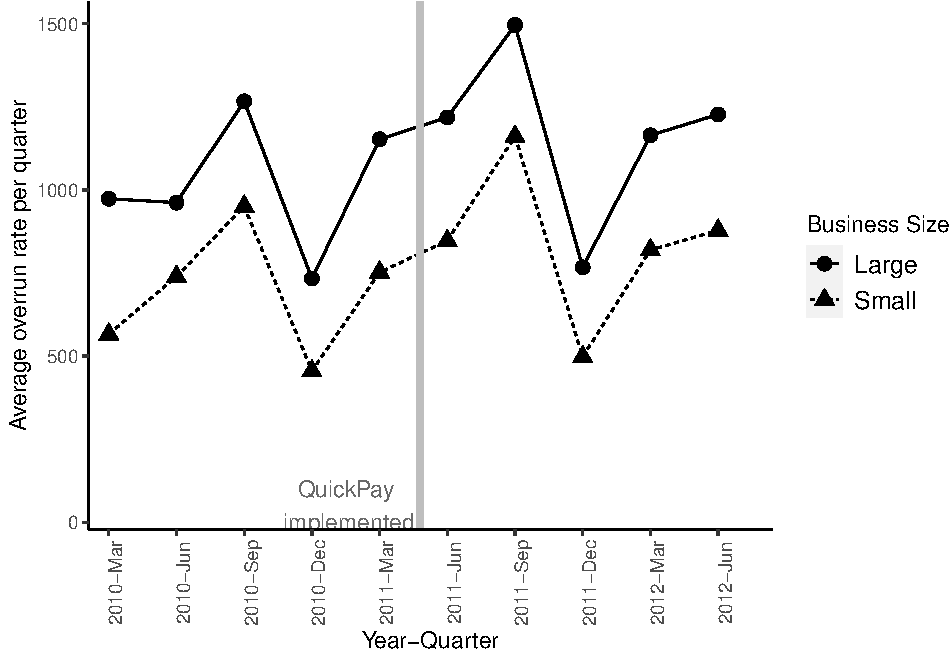
\includegraphics{qp_first_budget_overrun_files/figure-latex/plot-1.pdf}

\hypertarget{normalized-overrun}{%
\subsection{Normalized Overrun}\label{normalized-overrun}}

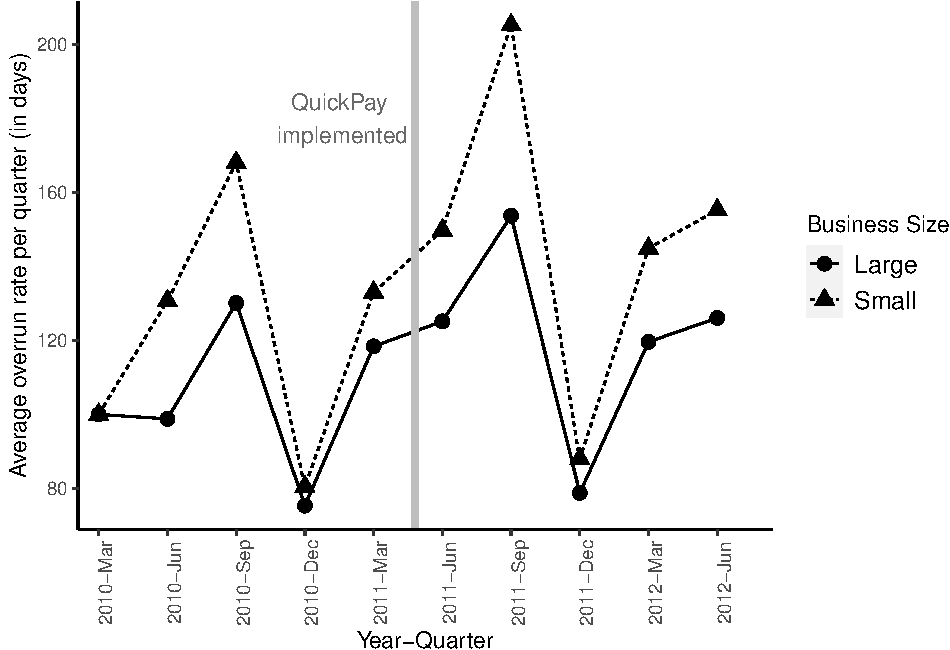
\includegraphics{qp_first_budget_overrun_files/figure-latex/normalized_plot-1.pdf}

\hypertarget{notation}{%
\section{Notation}\label{notation}}

\begin{itemize}
\tightlist
\item
  Project \(i\), Year-Quarter \(t\)
\item
  \(X_i\) denotes project level controls: initial duration, initial
  budget, number of offers received
\item
  \(\mu_t,\theta_{firm},\lambda_{task}\): Year-Quarter, Firm, and
  Product/Service code Fixed effects
\item
  All continuous variables are winsorized at the 5\% level
  \[ Treat_i = \begin{cases} 1, \text{ if project } i \text{ is a small business}\\
  0, \text{ otherwise} \end{cases}\]
  \[ Post_t = \begin{cases} 1, \text{ if year-quarter } t > \text{ April 27, 2011}\\
  0, \text{ otherwise} \end{cases}\]
\end{itemize}

\hypertarget{baseline-regressions}{%
\section{Baseline Regressions}\label{baseline-regressions}}

\[ Overrun_{it} = \alpha+\beta_0 Treat_i + \beta_1 Post_t + \beta_2 (Treat_i \times Post_t) + \epsilon_{it}\]

\[ \begin{aligned} Overrun_{it} &=& \alpha+\beta_0 Treat_i + \beta_1 Post_t + \beta_2 (Treat_i \times Post_t)\\
&+&  X_i + (Post_t \times X_i) + \mu_t + \theta_{firm} + \lambda_{task}+ \epsilon_{it}
\end{aligned}\]

\begin{table}[H] \centering 
  \caption{Quickpay 2009-2011} 
  \label{} 
\small 
\begin{tabular}{@{\extracolsep{-2pt}}lccccc} 
\\[-1.8ex]\hline 
\hline \\[-1.8ex] 
\\[-1.8ex] & \multicolumn{5}{c}{$Overrun_{it}$ (in days)} \\ 
\\[-1.8ex] & (1) & (2) & (3) & (4) & (5)\\ 
\hline \\[-1.8ex] 
 $Treat_i$ & $-$2,244.11$^{***}$ & $-$1,377.52$^{***}$ & $-$1,280.64$^{***}$ & $-$1,144.28$^{***}$ & $-$2,552.92$^{**}$ \\ 
  & (333.21) & (333.45) & (331.61) & (355.70) & (1,114.07) \\ 
  & & & & & \\ 
 $Post_t$ & 3,444.55$^{***}$ & $-$1,746.45$^{***}$ &  &  &  \\ 
  & (303.12) & (364.88) &  &  &  \\ 
  & & & & & \\ 
 $Treat_i \times Post_t$ & $-$1,323.31$^{***}$ & $-$710.86$^{*}$ & $-$731.80$^{*}$ & $-$559.47 & $-$371.98 \\ 
  & (400.76) & (407.64) & (405.93) & (406.24) & (438.97) \\ 
  & & & & & \\ 
 Constant & 9,543.11$^{***}$ & 2,405.81$^{***}$ &  &  &  \\ 
  & (249.87) & (647.47) &  &  &  \\ 
  & & & & & \\ 
\hline \\[-1.8ex] 
Duration, Budget, Bids & No & Yes & Yes & Yes & Yes \\ 
$Post_t \times$  (Duration, Budget, Bids) & No & Yes & Yes & Yes & Yes \\ 
Project Age Tercile & No & Yes & Yes & Yes & Yes \\ 
Year-Quarter Fixed Effects & No & No & Yes & Yes & Yes \\ 
Task Fixed Effects & No & No & No & Yes & Yes \\ 
Firm Fixed Effects & No & No & No & No & Yes \\ 
Observations & 127,056 & 117,671 & 117,671 & 117,671 & 117,671 \\ 
R$^{2}$ & 0.004 & 0.06 & 0.07 & 0.10 & 0.24 \\ 
Adjusted R$^{2}$ & 0.004 & 0.06 & 0.07 & 0.09 & 0.17 \\ 
\hline 
\hline \\[-1.8ex] 
\textit{Note:}  & \multicolumn{5}{r}{$^{*}$p$<$0.1; $^{**}$p$<$0.05; $^{***}$p$<$0.01} \\ 
 & \multicolumn{5}{r}{Each observation is a project-quarter.} \\ 
 & \multicolumn{5}{r}{SEs are robust and clustered at the project level.} \\ 
\end{tabular} 
\end{table}

\hypertarget{percentage-overrun}{%
\section{Percentage Overrun}\label{percentage-overrun}}

\[ PercentOverrun_{it} = \beta_0 + \beta_1 Treat_i + \beta_2 Post_t + \beta_3 (Treat_i \times Post_t) + e_{it}\]

\[ \begin{aligned} PercentOverrun_{it} &=& \alpha+\beta_0 Treat_i + \beta_1 Post_t + \beta_2 (Treat_i \times Post_t)\\
&+&  X_i + (Post_t \times X_i) + \mu_t + \theta_{firm} + \lambda_{task}+ \epsilon_{it}
\end{aligned}\]

\hypertarget{percentage-overrun-over-time}{%
\subsection{Percentage Overrun over
time}\label{percentage-overrun-over-time}}

\begin{itemize}
\tightlist
\item
  Sample restricted to projects with modification zero when they first
  appeared in our sample.
\item
  \(PercentOverrun_{it}=100 \times Overrun_{it}/Budget_{i,t-1}\)
\end{itemize}

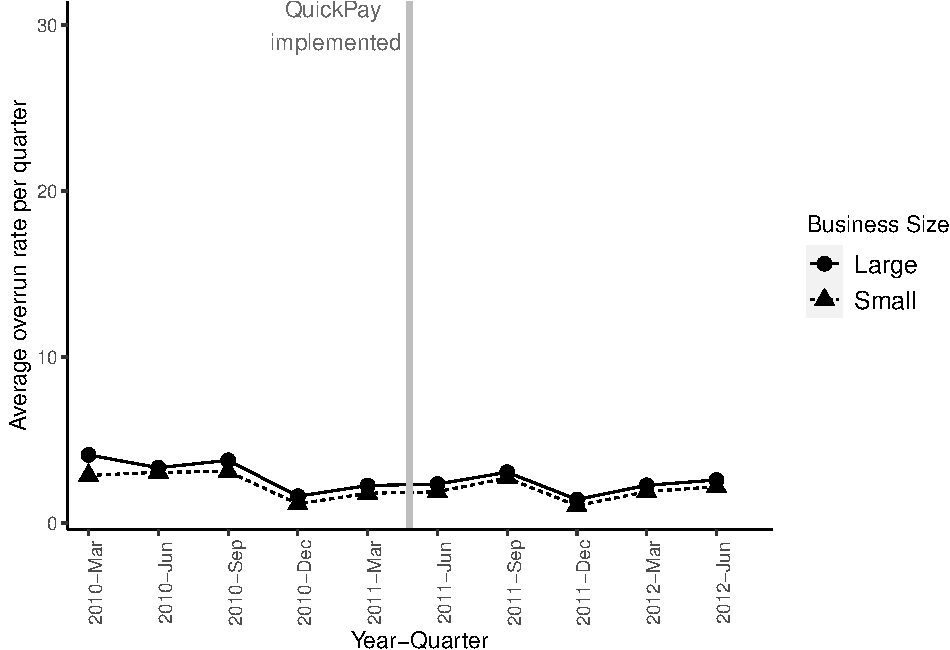
\includegraphics{qp_first_budget_overrun_files/figure-latex/plot_pc_overrun-1.pdf}

\hypertarget{normalized-overrun-1}{%
\subsubsection{Normalized Overrun}\label{normalized-overrun-1}}

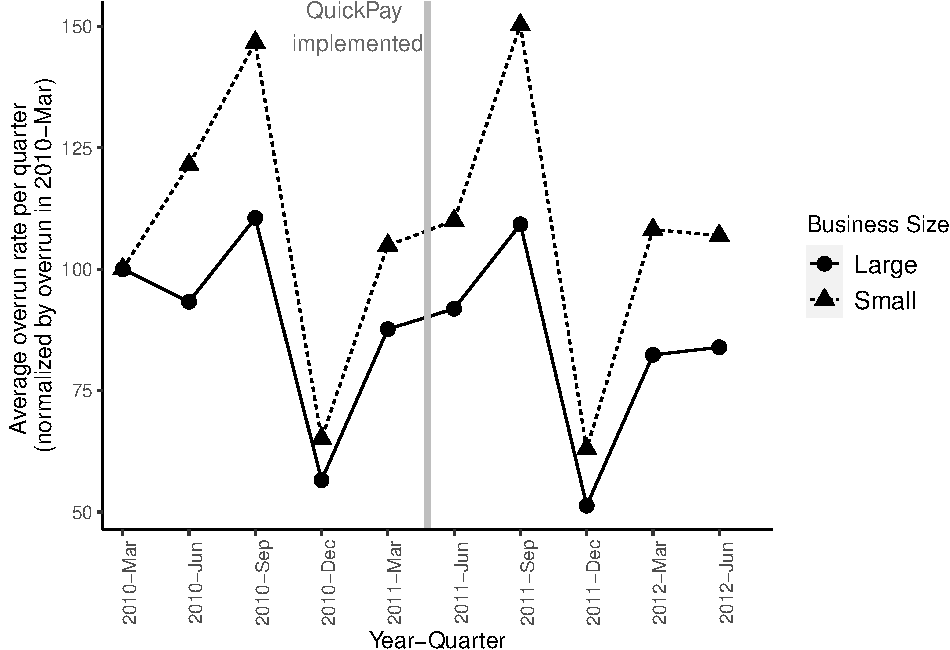
\includegraphics{qp_first_budget_overrun_files/figure-latex/normalized_pc_plot-1.pdf}

\begin{table}[H] \centering 
  \caption{Effect of QuickPay on project overrun rates} 
  \label{} 
\small 
\begin{tabular}{@{\extracolsep{-2pt}}lccccc} 
\\[-1.8ex]\hline 
\hline \\[-1.8ex] 
\\[-1.8ex] & \multicolumn{5}{c}{$PercentOverrun_{it}$} \\ 
\\[-1.8ex] & (1) & (2) & (3) & (4) & (5)\\ 
\hline \\[-1.8ex] 
 $Treat_i$ & $-$0.55$^{***}$ & $-$0.54$^{***}$ & $-$0.50$^{***}$ & $-$0.31$^{***}$ & $-$0.41 \\ 
  & (0.08) & (0.09) & (0.09) & (0.09) & (0.25) \\ 
  & & & & & \\ 
 $Post_t$ & $-$0.32$^{***}$ & $-$0.95$^{***}$ &  &  &  \\ 
  & (0.07) & (0.13) &  &  &  \\ 
  & & & & & \\ 
 $Treat_i \times Post_t$ & 0.15 & 0.11 & 0.09 & 0.10 & 0.12 \\ 
  & (0.10) & (0.10) & (0.10) & (0.10) & (0.11) \\ 
  & & & & & \\ 
 Constant & 2.61$^{***}$ & 4.19$^{***}$ &  &  &  \\ 
  & (0.06) & (0.17) &  &  &  \\ 
  & & & & & \\ 
\hline \\[-1.8ex] 
Duration, Budget, Bids & No & Yes & Yes & Yes & Yes \\ 
$Post_t \times$  (Duration, Budget, Bids) & No & Yes & Yes & Yes & Yes \\ 
Project age & No & Yes & Yes & Yes & Yes \\ 
Year-Quarter fixed effects & No & No & Yes & Yes & Yes \\ 
Task fixed effects & No & No & No & Yes & Yes \\ 
Contractor fixed effects & No & No & No & No & Yes \\ 
Observations & 124,419 & 116,240 & 116,240 & 116,240 & 116,240 \\ 
R$^{2}$ & 0.001 & 0.01 & 0.01 & 0.06 & 0.19 \\ 
Adjusted R$^{2}$ & 0.001 & 0.01 & 0.01 & 0.05 & 0.12 \\ 
\hline 
\hline \\[-1.8ex] 
\textit{Note:}  & \multicolumn{5}{r}{$^{*}$p$<$0.1; $^{**}$p$<$0.05; $^{***}$p$<$0.01} \\ 
 & \multicolumn{5}{r}{Each observation is a project-quarter.} \\ 
 & \multicolumn{5}{r}{SEs are robust and clustered at the project level.} \\ 
\end{tabular} 
\end{table}

\hypertarget{relative-overrun}{%
\section{Relative Overrun}\label{relative-overrun}}

\hypertarget{relative-overruns-over-time}{%
\subsection{Relative overruns over
time}\label{relative-overruns-over-time}}

\begin{itemize}
\item
  Sample restricted to projects with modification zero when they first
  appeared in our sample.
\item
  \(RelativeOverrun_{it} = 100 \times RelativeOverrun_{it}/IntialBudget_i\)
\end{itemize}

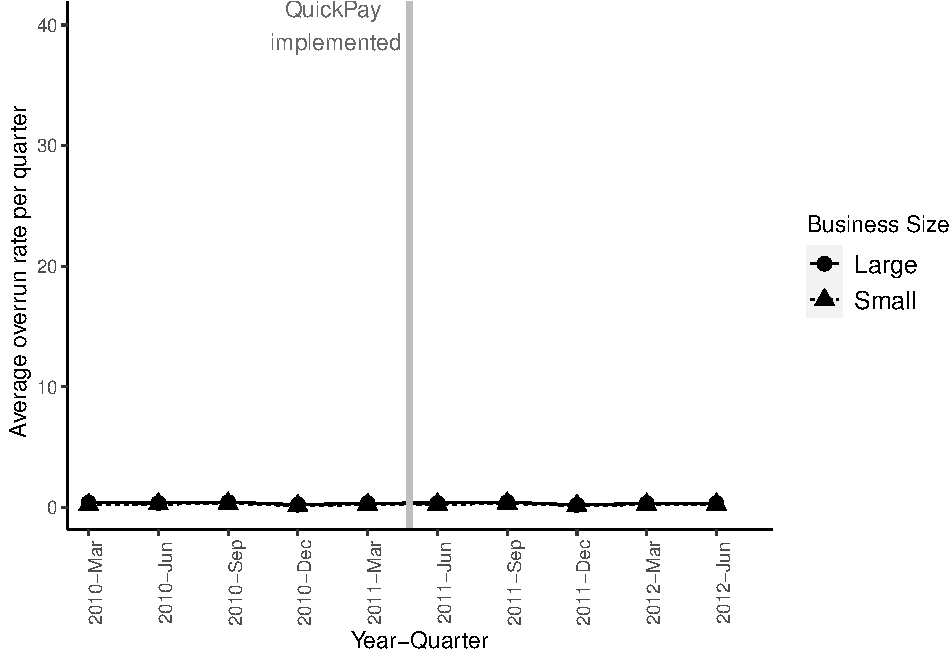
\includegraphics{qp_first_budget_overrun_files/figure-latex/plot_relative_overrun-1.pdf}

\hypertarget{normalized-overrun-2}{%
\subsubsection{Normalized overrun}\label{normalized-overrun-2}}

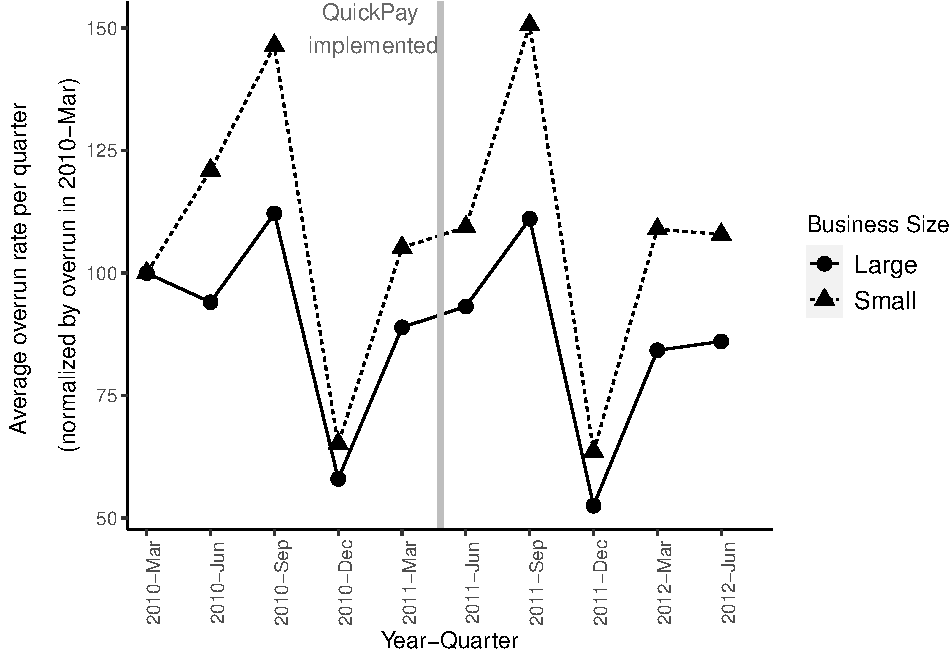
\includegraphics{qp_first_budget_overrun_files/figure-latex/normalized_relative_plot-1.pdf}

\begin{table}[H] \centering 
  \caption{Effect of QuickPay on project overrun rates} 
  \label{} 
\small 
\begin{tabular}{@{\extracolsep{-2pt}}lccccc} 
\\[-1.8ex]\hline 
\hline \\[-1.8ex] 
\\[-1.8ex] & \multicolumn{5}{c}{$RelativeOverrun_{it}$} \\ 
\\[-1.8ex] & (1) & (2) & (3) & (4) & (5)\\ 
\hline \\[-1.8ex] 
 $Treat_i$ & $-$0.69$^{***}$ & $-$0.60$^{***}$ & $-$0.57$^{***}$ & $-$0.32$^{***}$ & $-$0.65$^{**}$ \\ 
  & (0.10) & (0.10) & (0.10) & (0.11) & (0.31) \\ 
  & & & & & \\ 
 $Post_t$ & $-$0.24$^{***}$ & $-$0.92$^{***}$ &  &  &  \\ 
  & (0.08) & (0.14) &  &  &  \\ 
  & & & & & \\ 
 $Treat_i \times Post_t$ & 0.10 & 0.03 & 0.02 & 0.04 & 0.07 \\ 
  & (0.12) & (0.12) & (0.12) & (0.12) & (0.13) \\ 
  & & & & & \\ 
 Constant & 3.07$^{***}$ & 4.53$^{***}$ &  &  &  \\ 
  & (0.07) & (0.20) &  &  &  \\ 
  & & & & & \\ 
\hline \\[-1.8ex] 
Duration, Bids & No & Yes & Yes & Yes & Yes \\ 
$Post_t \times$  (Duration, Bids) & No & Yes & Yes & Yes & Yes \\ 
Project age & No & Yes & Yes & Yes & Yes \\ 
Year-Quarter fixed effects & No & No & Yes & Yes & Yes \\ 
Task fixed effects & No & No & No & Yes & Yes \\ 
Contractor fixed effects & No & No & No & No & Yes \\ 
Observations & 127,056 & 117,671 & 117,671 & 117,671 & 117,671 \\ 
R$^{2}$ & 0.001 & 0.004 & 0.01 & 0.06 & 0.20 \\ 
Adjusted R$^{2}$ & 0.001 & 0.004 & 0.01 & 0.05 & 0.12 \\ 
\hline 
\hline \\[-1.8ex] 
\textit{Note:}  & \multicolumn{5}{r}{$^{*}$p$<$0.1; $^{**}$p$<$0.05; $^{***}$p$<$0.01} \\ 
 & \multicolumn{5}{r}{Each observation is a project-quarter.} \\ 
 & \multicolumn{5}{r}{SEs are robust and clustered at the project level.} \\ 
\end{tabular} 
\end{table}

\end{document}
